\documentclass{standalone}
\usepackage{tikz}
\usetikzlibrary{patterns, positioning}
\usepackage[sfdefault]{ClearSans} %% option 'sfdefault' activates Clear Sans as the default text font
\usepackage[T1]{fontenc}

\begin{document}
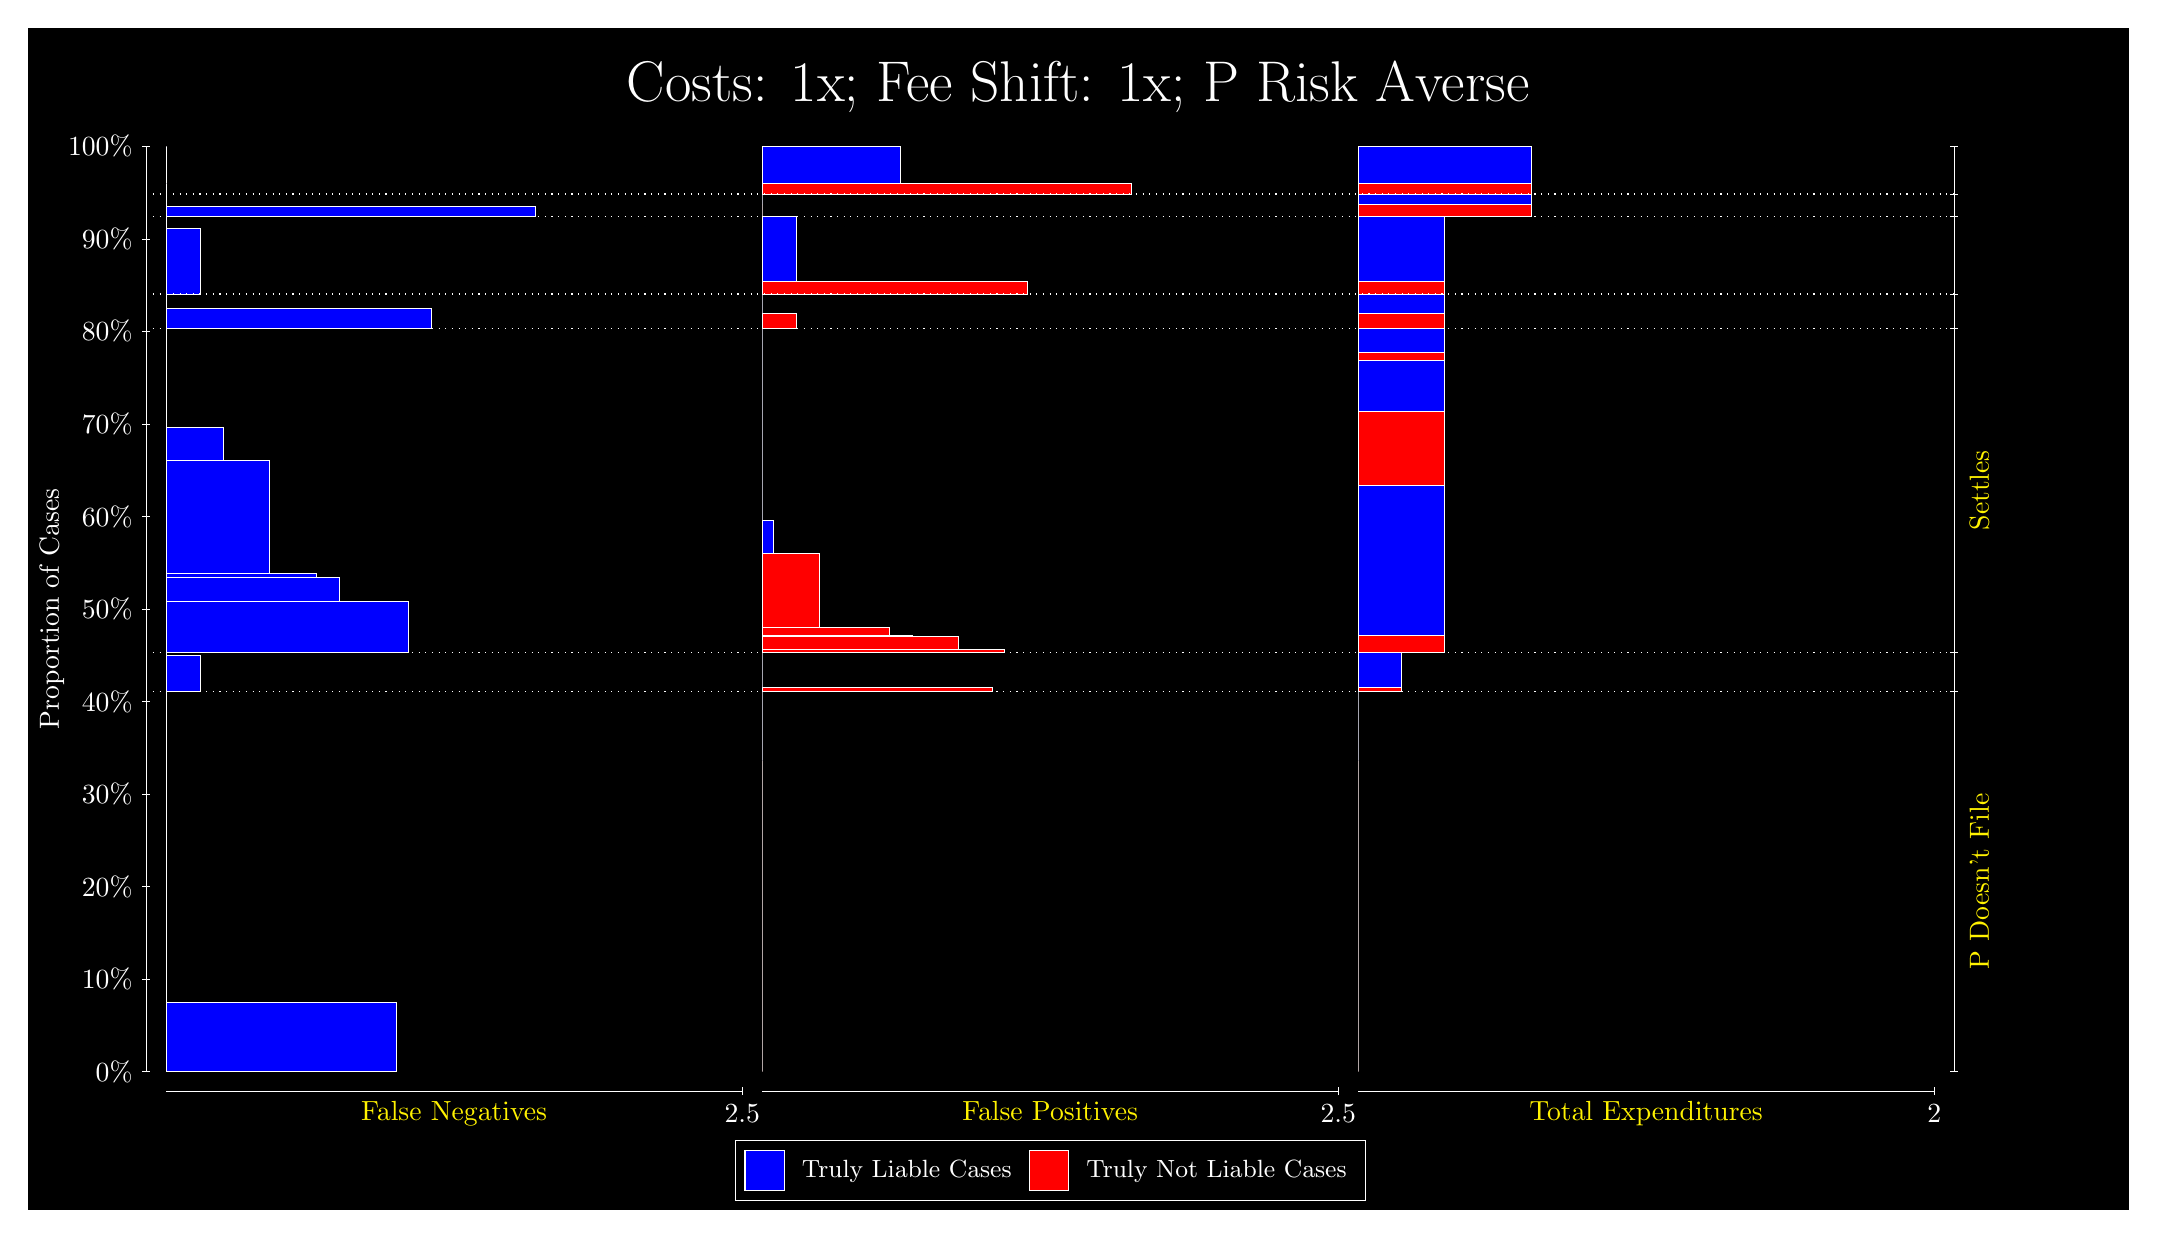
\begin{tikzpicture}
\draw[fill=black] (0,0) rectangle (26.667,15);
\draw[text=white] (0,13.5) rectangle (26.667,15) node[midway] {\huge Costs: 1x; Fee Shift: 1x; P Risk Averse};
\draw[white, very thin] (1.5,1.75) -- (1.5,13.5);
\node[rotate=90, text=white, anchor=center] at (0.3, 7.625) {Proportion of Cases};
\draw[white, very thin] (1.45,1.75) -- (1.55,1.75);
\node[text=white, anchor=east] at (1.45, 1.75) {0\%};
\draw[white, very thin] (1.45,2.925) -- (1.55,2.925);
\node[text=white, anchor=east] at (1.45, 2.925) {10\%};
\draw[white, very thin] (1.45,4.1) -- (1.55,4.1);
\node[text=white, anchor=east] at (1.45, 4.1) {20\%};
\draw[white, very thin] (1.45,5.275) -- (1.55,5.275);
\node[text=white, anchor=east] at (1.45, 5.275) {30\%};
\draw[white, very thin] (1.45,6.45) -- (1.55,6.45);
\node[text=white, anchor=east] at (1.45, 6.45) {40\%};
\draw[white, very thin] (1.45,7.625) -- (1.55,7.625);
\node[text=white, anchor=east] at (1.45, 7.625) {50\%};
\draw[white, very thin] (1.45,8.8) -- (1.55,8.8);
\node[text=white, anchor=east] at (1.45, 8.8) {60\%};
\draw[white, very thin] (1.45,9.975) -- (1.55,9.975);
\node[text=white, anchor=east] at (1.45, 9.975) {70\%};
\draw[white, very thin] (1.45,11.15) -- (1.55,11.15);
\node[text=white, anchor=east] at (1.45, 11.15) {80\%};
\draw[white, very thin] (1.45,12.325) -- (1.55,12.325);
\node[text=white, anchor=east] at (1.45, 12.325) {90\%};
\draw[white, very thin] (1.45,13.5) -- (1.55,13.5);
\node[text=white, anchor=east] at (1.45, 13.5) {100\%};

\draw[white, very thin] (24.457,1.75) -- (24.457,13.5);
\draw[white, very thin] (24.407,1.75) -- (24.507,1.75);
\node[anchor=west] at (24.407, 1.75) {};
\draw[white, very thin] (24.407,6.5784) -- (24.507,6.5784);
\node[anchor=west] at (24.407, 6.5784) {};
\draw[white, very thin] (24.407,7.0763) -- (24.507,7.0763);
\node[anchor=west] at (24.407, 7.0763) {};
\draw[white, very thin] (24.407,11.19) -- (24.507,11.19);
\node[anchor=west] at (24.407, 11.19) {};
\draw[white, very thin] (24.407,11.624) -- (24.507,11.624);
\node[anchor=west] at (24.407, 11.624) {};
\draw[white, very thin] (24.407,12.613) -- (24.507,12.613);
\node[anchor=west] at (24.407, 12.613) {};
\draw[white, very thin] (24.407,12.895) -- (24.507,12.895);
\node[anchor=west] at (24.407, 12.895) {};
\draw[white, very thin] (24.407,13.5) -- (24.507,13.5);
\node[anchor=west] at (24.407, 13.5) {};

\draw[white, very thin, fill=blue] (1.75,1.75) rectangle (4.6775,2.6291);
\draw[white, very thin, fill=red] (1.75,2.6291) rectangle (1.75,6.5784);
\draw[white, very thin, fill=blue] (1.75,6.5784) rectangle (2.1891,7.0304);
\draw[white, very thin, fill=red] (1.75,7.0304) rectangle (1.75,7.0763);
\draw[white, very thin, fill=blue] (1.75,7.0763) rectangle (4.8239,7.7253);
\draw[white, very thin, fill=blue] (1.75,7.7253) rectangle (3.9457,8.0298);
\draw[white, very thin, fill=blue] (1.75,8.0298) rectangle (3.6529,8.0839);
\draw[white, very thin, fill=blue] (1.75,8.0839) rectangle (3.0674,9.5158);
\draw[white, very thin, fill=blue] (1.75,9.5158) rectangle (2.4819,9.9374);
\draw[white, very thin, fill=red] (1.75,9.9374) rectangle (1.75,11.19);
\draw[white, very thin, fill=blue] (1.75,11.19) rectangle (5.1167,11.44);
\draw[white, very thin, fill=red] (1.75,11.44) rectangle (1.75,11.624);
\draw[white, very thin, fill=blue] (1.75,11.624) rectangle (2.1891,12.454);
\draw[white, very thin, fill=red] (1.75,12.454) rectangle (1.75,12.613);
\draw[white, very thin, fill=blue] (1.75,12.613) rectangle (6.4341,12.744);
\draw[white, very thin, fill=red] (1.75,12.744) rectangle (1.75,12.895);
\draw[white, very thin, fill=red] (1.75,12.895) rectangle (1.75,13.027);
\draw[white, very thin, fill=blue] (1.75,13.027) rectangle (1.75,13.5);
\draw[white, very thin, fill=red] (9.3189,1.75) rectangle (9.3189,5.6993);
\draw[white, very thin, fill=blue] (9.3189,5.6993) rectangle (9.3189,6.5784);
\draw[white, very thin, fill=red] (9.3189,6.5784) rectangle (12.246,6.6243);
\draw[white, very thin, fill=blue] (9.3189,6.6243) rectangle (9.3189,7.0763);
\draw[white, very thin, fill=red] (9.3189,7.0763) rectangle (12.393,7.1132);
\draw[white, very thin, fill=red] (9.3189,7.1132) rectangle (11.807,7.2809);
\draw[white, very thin, fill=red] (9.3189,7.2809) rectangle (11.222,7.2923);
\draw[white, very thin, fill=red] (9.3189,7.2923) rectangle (10.929,7.3971);
\draw[white, very thin, fill=red] (9.3189,7.3971) rectangle (10.051,8.3293);
\draw[white, very thin, fill=blue] (9.3189,8.3293) rectangle (9.4652,8.7509);
\draw[white, very thin, fill=blue] (9.3189,8.7509) rectangle (9.3189,11.19);
\draw[white, very thin, fill=red] (9.3189,11.19) rectangle (9.758,11.374);
\draw[white, very thin, fill=blue] (9.3189,11.374) rectangle (9.3189,11.624);
\draw[white, very thin, fill=red] (9.3189,11.624) rectangle (12.686,11.784);
\draw[white, very thin, fill=blue] (9.3189,11.784) rectangle (9.758,12.613);
\draw[white, very thin, fill=red] (9.3189,12.613) rectangle (9.3189,12.765);
\draw[white, very thin, fill=blue] (9.3189,12.765) rectangle (9.3189,12.895);
\draw[white, very thin, fill=red] (9.3189,12.895) rectangle (14.003,13.027);
\draw[white, very thin, fill=blue] (9.3189,13.027) rectangle (11.075,13.5);
\draw[white, very thin, fill=red] (16.888,1.75) rectangle (16.888,5.6993);
\draw[white, very thin, fill=blue] (16.888,5.6993) rectangle (16.888,6.5784);
\draw[white, very thin, fill=red] (16.888,6.5784) rectangle (17.437,6.6243);
\draw[white, very thin, fill=blue] (16.888,6.6243) rectangle (17.437,7.0763);
\draw[white, very thin, fill=red] (16.888,7.0763) rectangle (17.986,7.2923);
\draw[white, very thin, fill=blue] (16.888,7.2923) rectangle (17.986,9.1999);
\draw[white, very thin, fill=red] (16.888,9.1999) rectangle (17.986,10.132);
\draw[white, very thin, fill=blue] (16.888,10.132) rectangle (17.986,10.781);
\draw[white, very thin, fill=red] (16.888,10.781) rectangle (17.986,10.886);
\draw[white, very thin, fill=blue] (16.888,10.886) rectangle (17.986,11.19);
\draw[white, very thin, fill=red] (16.888,11.19) rectangle (17.986,11.374);
\draw[white, very thin, fill=blue] (16.888,11.374) rectangle (17.986,11.624);
\draw[white, very thin, fill=red] (16.888,11.624) rectangle (17.986,11.784);
\draw[white, very thin, fill=blue] (16.888,11.784) rectangle (17.986,12.613);
\draw[white, very thin, fill=red] (16.888,12.613) rectangle (19.083,12.765);
\draw[white, very thin, fill=blue] (16.888,12.765) rectangle (19.083,12.895);
\draw[white, very thin, fill=red] (16.888,12.895) rectangle (19.083,13.027);
\draw[white, very thin, fill=blue] (16.888,13.027) rectangle (19.083,13.5);
\draw[white, dotted] (1.5,6.5784) -- (24.457,6.5784);
\draw[white, dotted] (1.5,7.0763) -- (24.457,7.0763);
\draw[white, dotted] (1.5,11.19) -- (24.457,11.19);
\draw[white, dotted] (1.5,11.624) -- (24.457,11.624);
\draw[white, dotted] (1.5,12.613) -- (24.457,12.613);
\draw[white, dotted] (1.5,12.895) -- (24.457,12.895);
\draw[white, very thin] (1.75,1.5) -- (9.0689,1.5);
\node[text=yellow, anchor=north] at (5.4094, 1.5) {False Negatives};
\draw[white, very thin] (9.0689,1.45) -- (9.0689,1.55);
\node[text=white, anchor=north] at (9.0689, 1.45) {2.5};

\draw[white, very thin] (9.3189,1.5) -- (16.638,1.5);
\node[text=yellow, anchor=north] at (12.978, 1.5) {False Positives};
\draw[white, very thin] (16.638,1.45) -- (16.638,1.55);
\node[text=white, anchor=north] at (16.638, 1.45) {2.5};

\draw[white, very thin] (16.888,1.5) -- (24.207,1.5);
\node[text=yellow, anchor=north] at (20.547, 1.5) {Total Expenditures};
\draw[white, very thin] (24.207,1.45) -- (24.207,1.55);
\node[text=white, anchor=north] at (24.207, 1.45) {2};

\node[text=yellow, centered, rotate=90] at (24.777, 4.1642) {P Doesn't File};

\node[text=yellow, centered, rotate=90] at (24.777, 9.1333) {Settles};





\draw (12.978300999999998,1.5) node[draw=none] (baseCoordinate) {};
\begin{scope}[align=center]
        \matrix[scale=0.5, draw=white, below=0.5cm of baseCoordinate, nodes={draw}, column sep=0.1cm]{
            \node[rectangle, draw, minimum width=0.5cm, minimum height=0.5cm, fill=blue] {}; &
            \node[draw=none, font=\small, text=white] (B) {Truly Liable Cases}; &
            \node[rectangle, draw, minimum width=0.5cm, minimum height=0.5cm, fill=red] {}; &
            \node[draw=none, font=\small, text=white] (B) {Truly Not Liable Cases}; \\
            };
\end{scope}

\end{tikzpicture}
\end{document}